\documentclass[tikz,border=0cm,dvipsnames,x11names,rgb]{standalone}

\usepackage{amsmath,amssymb,amsfonts}
\usetikzlibrary{calc,
fit,
shapes.misc,
shapes.geometric,
arrows.meta,
fadings,
matrix,
chains,
scopes,
positioning}

\usepackage{pgfplots}
\usepackage{pgfplotstable}
\pgfplotsset{compat=1.18}



\usepackage[]{fontspec}

\setmainfont{Latin Modern Roman}
\setmonofont{Latin Modern Math}
\renewcommand{\textsc}[1]{{\fontfamily{lmr}\selectfont \scshape #1}}

\usepackage[]{bm}

\makeatletter
\@ifundefined{fromRoot}{\newcommand{\fromRoot}[1]{../../#1}}{}

\def\input@path{{../..}{..}{.}{./svg}{./pgfplots}{./tikzpicture}}
%or: \def\input@path{{/path/to/folder/}{/path/to/other/folder/}}
\makeatother

\newcommand{\ra}[1]{\renewcommand{\arraystretch}{#1}}

\newcommand*{\gf}[1]{\acrshort{gf}($#1$)}%
\newcommand*{\mpn}[1]{\bm{P}_{#1}}%
\newcommand*{\pn}[1]{%
  \ifthenelse{\equal{#1}{}}{$\mpn{0}$}{$\mpn{#1}$}%
}%

\newcommand*{\pk}[3]{%
  \ifthenelse{\equal{#1}{#2}}{\textcolor{red}{\phantom{.}$p_0$\phantom{.}}}{\phantom{.}$p_#3$\phantom{.}}%
}%


\newcommand*{\placeholderreg}{\includegraphics[width=\linewidth, height=.25\textheight, keepaspectratio = true]{figures/certified_xilinx.png}}%
\newcommand*{\placeholder}[1]{\includegraphics[#1]{figures/certified_xilinx.png}}%

\newcommand*{\snr}{\acrshort{snr}}%
\newcommand*{\snrs}{\acrshortpl{snr}}%

\newcommand*{\mpd}[0]{p_\Delta}%
\newcommand*{\mpo}[0]{p_\omega}%
\newcommand*{\pd}[0]{$\mpd$}%
\newcommand*{\po}[0]{$\mpo$}%
\newcommand*{\mpfa}[0]{\mathcal{P}_{fa}}%
\newcommand*{\mpmd}[0]{\mathcal{P}_{md}}%
\newcommand*{\pfa}[0]{\acrshort{pfa}}%
\newcommand*{\pmd}[0]{\acrshort{pmd}}%
\newcommand*{\mnorm}[1]{\mathcal{L}_{#1}}%
\newcommand*{\norm}[1]{$\mnorm{#1}$}%
\newcommand*{\fft}{\acrshort{fft}}%
\newcommand*{\mfft}[1]{\mathcal{F}(#1)}%
\newcommand*{\mifft}[1]{\mathcal{F}^{-1}(#1)}%
\newcommand*{\ts}{\acrshort{ts}}%

\newcommand*{\cpp}[1]{C\textrm{++#1}}%
\newcommand*{\na}{\textrm{\textcolor{SlateGray4}{N/A}}}%

\newcommand*{\vect}[1]{\bm{#1}}%
\newcommand*{\mat}[1]{\bm{\mathrm{#1}}}%

\newcommand*{\task}[1]{\mathcal{T}_{#1}}%

\newcommand*{\sdr}{\acrshort{sdr}}%
\newcommand*{\fpga}{\acrshort{fpga}}%

\newcommand*{\rikiki}{\fontsize{4}{6}\selectfont}%




\begin{document}
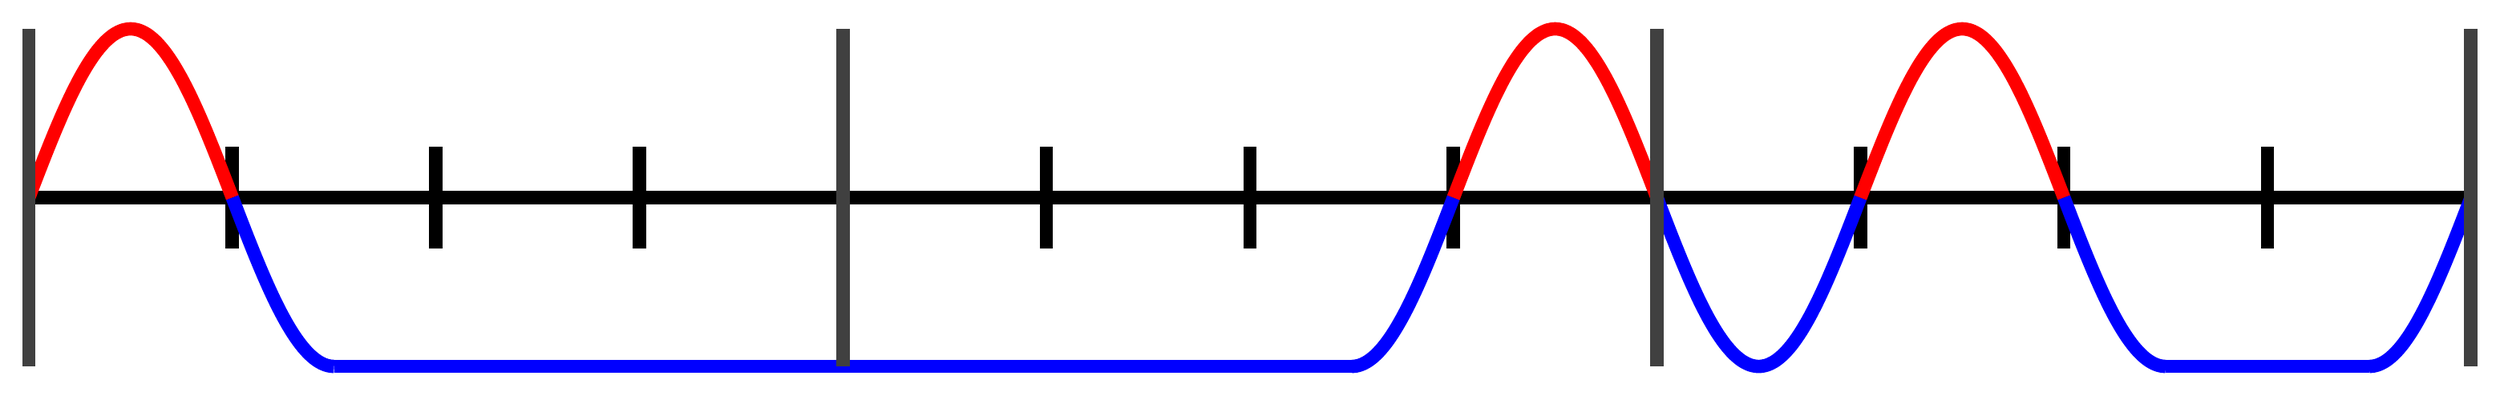
\begin{tikzpicture}[
    line width = 2pt,
    every node/.style = {font={\large}}
  ]
  % {0, 3, 1}

  % 0
  % \draw [Red] (0, 0) -- (0.25, 1);
  % \draw [Red] (0.25, 1) -- (.75, 1);
  % \draw [Red] (.75, 1) -- (1, 0);
  % \draw [Blue] (1, 0) -- (1.25, -1);
  % \foreach \t [
  %   evaluate = \t as \tt using (\t + .25),
  %   evaluate = \t as \tp1 using (\t + 1.25)
  % ] in {1, ..., 5}
  %   {
  %     \draw [Blue] (\tt, -1) -- (\tp1, -1);
  %   }
  % \draw [Blue] (6.25, -1) -- (6.75, -1);
  % \draw [Blue] (6.75, -1) -- (7, 0);

  % \draw [Red] (7, 0) -- (7.25, 1);
  % \draw [Red] (7.25, 1) -- (7.75, 1);
  % \draw [Red] (7.75, 1) -- (8, 0);

  % \draw [Blue] (8, 0) -- (8.25, -1);
  % \draw [Blue] (8.25, -1) -- (8.75, -1);
  % \draw [Blue] (8.75, -1) -- (9, 0);

  % \draw [Red] (9, 0) -- (9.25, 1);
  % \draw [Red] (9.25, 1) -- (9.75, 1);
  % \draw [Red] (9.75, 1) -- (10, 0);

  % \draw [Blue] (10, 0) -- (10.25, -1);
  % \foreach \t [
  %   evaluate = \t as \tt using (\t + .25),
  %   evaluate = \t as \tp1 using (\t + 1.25)
  % ] in {10, 11}
  %   {
  %     \draw [Blue] (\tt, -1) -- (\tp1, -1);
  %   }
  % \draw [Blue] (12.25, -1) -- (12.75, -1);
  % \draw [Blue] (12.75, -1) -- (13, 0);

  % \draw [dashed,line width = 3pt, darkgray] (4, 0) -- (4, 1);
  % \draw [dashed,line width = 3pt, darkgray] (8, 0) -- (8, 1);

  \begin{axis} [
      hide axis,
      mark = none,
      line width = 6pt,
      % grid on,
      height = 8 cm,
      width  = 48cm,
    ]

    \draw [solid, black] (0, 0) -- (12, 0);
    \foreach \t in {0, ..., 12} {
        \edef\temp{\noexpand\draw (\t, .3) -- (\t, -.3);}
        \temp
      }

    \addplot [Red, smooth, domain = 0:1] {sin(deg(x * pi))};
    \addplot [Blue, smooth, domain = 1:1.5] {sin(deg(x * pi))};
    \addplot [Blue, smooth, domain = 1.5:6.5] {-1};
    \addplot [Blue, smooth, domain = 6.5:7] {-sin(deg(x * pi))};
    \addplot [Red, smooth, domain = 7:8] {-sin(deg(x * pi))};
    \addplot [Blue, smooth, domain = 8:9] {-sin(deg(x * pi))};
    \addplot [Red, smooth, domain = 9:10] {-sin(deg(x * pi))};
    \addplot [Blue, smooth, domain = 10:10.5] {-sin(deg(x * pi))};
    \addplot [Blue, smooth, domain = 10.5:11.5] {-1};
    \addplot [Blue, smooth, domain = 11.5:12] {sin(deg(x * pi))};


    \foreach \t in {0, 4, ..., 12} {
        \edef\temp{\noexpand\draw [darkgray] (\t, 1) -- (\t, -1);}
        \temp
      }
  \end{axis}

\end{tikzpicture}
\end{document}
